\documentclass[a4paper,12pt,headsepline,pagesize,bibtotoc,titlepage]{scrartcl}

\usepackage{scrpage2}
\pagestyle{useheadings}
\usepackage[english]{babel}
\usepackage[utf8]{inputenc}

\usepackage[T1]{fontenc}

\usepackage{mathptmx}
\usepackage[scaled=.90]{helvet}
\usepackage{courier}

\usepackage{amsmath,amsthm,amsfonts,graphicx,caption}

\usepackage{hyperref}   % Clickable hyperlinks
\usepackage{ae,aecompl} % Better fonts for the screen

\headsep4mm

\typearea[current]{current}

\renewcommand{\figurename}{Fig.}
\renewcommand{\captionlabelfont}{\bf}

\title{
	\includegraphics*[width=0.4\textwidth]{images/hpi_logo.png}\\
	\vspace{24pt}
	Deep Learning for Video Classification
}

\subtitle{
	Master’s project\\
	Internet Technologies and Systems\\
	Summer semester 2015
}
\author{
	Tanja Bergmann, Joseph Bethge, Tom Bocklisch, \\
	Stefan Bunk, Tom Herold, Dominik Mueller \\ \\[12pt]
	Supervisor:\\
	Dr. Haojin Yang\\
	Prof. Dr. Christoph Meinel
}
\date{\today}
\begin{document}
\maketitle
\tableofcontents
\newpage

\section{Introduction}
\label{sec:introduction}

This research report summarizes our experiences and experiments for activity recognition in videos using the deep neural network framework Caffe~\cite{jia2014caffe}.

Section~\ref{sec:related} lists and summarizes the papers we built on.
We also talk about our problems reproducing some of their results.
Section~\ref{sec:data} shows the details of our data preprocessing.
Section~\ref{sec:classification} explains our net architectures and shows the results of some experiments.
Section~\ref{sec:web} focuses on the web application, and finally section~\ref{sec:scripts} summarizes the scripts we used and implemented during our work.

\subsection{Research Task}
The goal of this research project is to apply state of the art deep neural network to activity recognition for videos.
We aim to confirm the outstanding classification performance of a two-stream learning architecture~\cite{simonyan2014two} as proposed by Simonyan et al.
More specifically, we focus on validating the top of the class prediction results of 91.3\% as presented by Wu et al.~\cite{wu2015modeling}.


%!TEX root = ../paper.tex
\section{Related Work}
\label{sec:related}

\begin{itemize}
	\item Explain the development in the last two years and their respective approaches
	\item Explain, why some papers are hard to reproduce
\end{itemize}

\subsection*{Reproducibility Issues}
Some papers were hard to reproduce, because the data generation was not described in detail.
Concretely, these are parameters, which were not mentioned (neither in the paper nor on the web page) for some approaches:
\begin{itemize}
	\item Which frame rate was used to extract frames from videos
	\item When frames are sampled from the video, which selection schema was used?
	\item
	\item IDEA: Use a table and list which paper lists which preprocessing steps?
	\item TODO
\end{itemize}

%!TEX root = ../paper.tex
\section{Data Preparation}
\label{sec:data}

As mentioned in Section~\ref{sec:related}, there are many parameters and design decisions in the data generation and preparation process, which influence the final performance.
This section discusses all these parameters in detail.
In general we first extract the frame images from a video, and then calculate optical flow images based on two adjacent frames.
This captures the movement between those two frames.
After the data generation, the preprocessed data has to be converted into a suitable data file for the Caffe framework.
In the following section we will discuss the different ways and data formats available for each step in detail.

\subsection{Dataset}
For our research purposes we relied on the UCF101~\cite{soomro2012ucf101} dataset, a popular choice in the computer vision community.
UCF101 is an action recognition data set of realistic action videos, collected from YouTube, having 101 action categories.
The videos in the 101 action categories are grouped into 25 groups, where each group can consist of 4-7 video clips of an action.
The videos from the same group may share some common features, such as similar background, similar viewpoint, etc.
The action categories can be divided into five types:
\begin{enumerate*}
	\item Human-Object Interaction
	\item Body-Motion Only
	\item Human-Human Interaction
	\item Playing Musical Instruments
	\item Sports.
\end{enumerate*}
The dataset contains of 13320 clips with a fixed frame rate and a resolution of \texttt{320 x 240} respectively.
There are a few videos in the \emph{PommelHorse} category, which have a different resolution of \texttt{400 x 226}.
We dealt with these by rescaling them to \texttt{320 x 240}.
On average the clips have a length of 7 seconds.

For comparable results the dataset's authors published three fixed train/test splits.
We worked on the first split, i.e. \texttt{trainlist01.txt} and \texttt{testlist01.txt}\footnote{ \url{http://crcv.ucf.edu/data/UCF101/UCF101TrainTestSplits-RecognitionTask.zip}}.
When working with UC101 it is important to follow these splits, because training instances are often sampled and cut from a longer video sequence.
Concretely, this means that dataset's authors gathered long activity video sequences and cut them into short clips to create more than one training sample from this sequence.
It is important to keep the samples from one original sequence in the same dataset or otherwise the test performance is estimated too high.

\subsection{Frame extraction}
The first preprocessing step needs to convert the given \texttt{*.avi} video files into single-frame pictures.
We extracted the frame data from the videos with the \emph{FFmpeg}\footnote{\url{http://www.ffmpeg.org}} tool.
See Section~\ref{subsec:frame_extraction} for the concrete parameters.
As output, we chose JPEG files.
Finding the correct frame rate for the frame extraction was challenging.
High frame rates, such as 30 frames per second, often lead to two adjacent frames being exactly identical.
This is a problem for the optical flow extraction, since there will be almost no measurable difference between the images and the optical flow is reported as empty.
Especially for classes, where a lot of movement and characteristic optical flow is expected (such as \emph{Archery} or \emph{Juggling Balls}), this turned out to be problematic.
The problem of identical images does not exist for lower frame rates, e.g. 5 frames per second.
However in this case we create less overall training data and less details, especially for optical flow extraction.
A variable frame rate extraction is not feasible, as the optical flow must be comparable between different video types, i.e. the time between two frames must be identical.
This is why we decided to use a fixed frame rate of 15 frames per second.
% COMMENT: The data on the server is definitely 15 frames per second. There are twice as much frames in the frames_30fps/ subfolders than in the frames/ subfolders.
This minimized the occurrence of two identical adjacent frames while still giving a sufficient amount of detail.

\subsection{Optical flow extraction}
Optical flow is computed to capture the movement in a video sequence and is always based on two immediate consecutive grey-scale frames.
We used the optical flow algorithm from Brox et al~\cite{brox2004high}, an accepted standard in the research community.
We were able to apply the out of the box OpenCV algorithm \footnote{\url{http://docs.opencv.org/modules/gpu/doc/video.html\#gpu-broxopticalflow}} and benefited from its GPU computation, leading to faster flow extraction.
Optical flow can be computed both along X and Y axis. Therefore there are two optical flow images for each pair of consecutive frames, resulting in $2 * (N - 1)$ optical flows for $N$ frames.

\todo{Figure}

\subsection{Optical flow frame stacking}
A single optical flow image does not contain as much information as the RGB picture of the same frame.
Therefore, several optical flow images are stacked, just as the color channels \emph{R}, \emph{G}, and \emph{B} are stacked in a standard image.
For each frame, we stack the optical flows for the next 10 frames in both X and Y direction, leading to a total stack size of 20.
We experimented with adding the flows of the 10 previous frames as well, leading to a stack size of 40.
However, this did not improve the results.\todo{könnte es sein, dass wir das gemacht haben, als das Stacking noch kaputt war?}
Note, stacking is done with a sliding window. E.g. we add the optical flows from the \nth{1} to the \nth{2} frame, from the \nth{2} to the \nth{3} frame, and so on. X and Y flows are interleaved.


\subsection{Data format for caffe}
% Experiences with LMDB, LevelDB, HDF5
The caffe framework accepts different formats for the input data. Commonly the data is stored in a database of the type LMDB, HDF5, or LevelDB.
In our initial tests, we used LMDB, as this is usually used in the Caffe examples, and seems to be the recommended option.
Using LMDB resulted in very large databases, because it does not support compression.
This led to disk space issues.

We went on to use HDF5, which compresses the data.
However, we relied on the Python library h5py\footnote{\url{http://www.h5py.org/}}, which turned out to have major memory leaks.
Therefore, we cannot recommend using HDF5 in Python environment.
The library was consuming so much RAM and swap space, that the machine had to be killed at times.
Also, the Caffe documentation states, that HDF5 should only be used ``when efficiency is not critical''.

Finally we settled on LevelDB, a database developed by Google for fast read performance.
Compression is done using Google's Snappy\footnote{\url{http://google.github.io/snappy/}} library, which offers both good performance and compression.
We therefore recommend LevelDB. A complete comparison of the DB creation time and size can be found in table \ref{table:databases}.

\todo{Who has the table values?}
\begin{table}[H]
\centering
\caption{Data format comparison}
\label{table:databases}
\begin{tabular}{lll}
\toprule
Creation Time 		& DB Size  & DB Type \\ \midrule
TODO           & XX GB  	 & LMDB \\
TODO          		& XX GB  	 & HDF5 \\
TODO          		& XX GB  	 & LevelDB \\
\bottomrule
\end{tabular}
\end{table}

\subsection{Image cropping}
As mentioned before, most images have a resolution of \texttt{320 x 240}.
On the other hand, most convolutional network architectures require a squared input resolution.
The \emph{Caffenet} requires data to be in \texttt{227 x 227}, the \emph{CNN\_M} network requires a resolution of \texttt{224 x 224}.
The best approach to transform an image from its original resolution to the required resolution is cropping.
Caffe already comes with a built-in method for randomly cropping images.
When setting the \texttt{crop\_size} parameter in the net definition, the input image is cropped randomly every time the image is read for training or testing.
Also, mirroring can be used to further increase the training size with the same approach.

Some authors~\cite{ye2015evaluating} perform this cropping manually, by taking a clipping from each corner and from the center of the image. (see section \ref{subsec:crop_mirror_frames})
We also tried this approach, but discarded it from our final setup, because of two reasons.
Firstly, it massively increases the training set size making the data harder to handle and requiring more disk space.
Secondly, the random cropping in Caffe is at least as effective \todo{effective ist hier ungenau (bedeutung), ausserdem hilft das feste cropping mit der Varianz der Bilder, da caffe oft in der mitte cropped} as manually cropping and can save us some work.

\subsection{Selecting frames for the LSTM}
For the LSTMs, we need another set of databases (spatial and flow), which contain only a fixed number of frames per video.
We decided to use 16 frames per video, on the grounds that the LSTM implementation \footnote{\url{https://github.com/jeffdonahue/caffe/tree/recurrent}} by Jeff Donahue cannot handle arbitrarily long input sequences, especially over batches.
From every videos' frame pool we selected these 16 frames by omitting the first and last five frames\todo{Ich glaube, das machen wir nicht mehr}, and the equally distributing the selected frames among the remaining frames.
By skipping some frames at the beginning and end, we avoided the fade-in/fade-out effects in some of the videos.
For details on how to create such a selection see section \ref{subsec:listfile_to_file_ucf_static}.
Additionally, these sets of frames are used for training the fusion network.

\subsection{Relevant scripts}

\subsubsection{convert\_imageset}
A Caffe utility to bundle a list of individual images into a database file. Supports both LMDB and LevelDB.

\begin{table}[H]
\begin{tabularx}{\textwidth}{p{0.5cm}p{3cm}L}
\multicolumn{2}{l}{Location}  		& \textit{caffe/build/tools/} \\
\multicolumn{2}{l}{Parameter} 		&                                        \\
        & \textit{root\_folder}		& the root folder from where to search for the videos in the file list  \\
        & \textit{file\_list}		& a text file containing one file path to a video and its class per line \\
        & \textit{database\_name}   & the name and path of the newly created DB \\
        & \textit{-backend}    		& switches between \textit{leveldb} and \textit{lmdb}  \\
\multicolumn{2}{l}{Example}  		& \textit{convert\_imageset -backend leveldb /opt/data\_sets/UCF101 filelist.txt /opt/data\_sets/UCF101/leveldb.leveldb} \\        
\end{tabularx}
\end{table}

\subsubsection{convert\_imageset\_multi}
\label{subsec:convert_imageset_multi}
A slight modification to the original \texttt{convert\_imageset} to allow for stacking a number of images into a single data structure before storing them in a database file. Otherwise identical to original above. Note, this script is only available in our Caffe fork.

\begin{table}[H]
\begin{tabularx}{\textwidth}{p{0.5cm}p{3cm}L}
\multicolumn{2}{l}{Location}  		& \textit{caffe/build/tools/} \\
\multicolumn{2}{l}{Parameter} 		&                                        \\
        & \textit{root\_folder}		& the root folder from where to search for the videos in the file list  \\
        & \textit{file\_list}		& a text file containing one file path to a video and its class per line \\
        & \textit{database\_name}   & the name and path of the newly created DB \\
        & \textit{stack\_size}    	& a number indicating how many succeeding images from the list will be merged \\
        & \textit{-backend}    		& switches between \textit{leveldb} and \textit{lmdb} \\
\multicolumn{2}{l}{Example}  		& \textit{convert\_imageset\_multi -backend leveldb /opt/data\_sets/UCF101 filelist.txt /opt/data\_sets/UCF101/leveldb.leveldb 16} \\        
\end{tabularx}
\end{table}

\subsubsection{frame\_extraction.sh}
\label{subsec:frame_extraction}
A wrapper around \textit{ffmpeg } responsible for extracting the image frames from all UCF101 video files.

\begin{table}[H]
\begin{tabularx}{\textwidth}{p{0.5cm}p{3cm}L}
\multicolumn{2}{l}{Location}  		& \textit{video-classification/tools/} \\
\multicolumn{2}{l}{Parameter} 		&                                        \\
        & \textit{input\_folder}	& the root folder containing all the UCF101 videos  \\
        & \textit{output\_folder}	& the root folder for storing the extracted frames \\
        & \textit{frame\_rate}  	& the frame rate for extraction \\
\multicolumn{2}{l}{Example}  		& \textit{frame\_extraction.sh /opt/data\_sets/UCF-101/videos/ /opt/data\_sets/UCF-101/frames\_10fps/ 10} \\        
\end{tabularx}
\end{table}


\subsubsection{listfile\_to\_file\_ucf\_static.py}
\label{subsec:listfile_to_file_ucf_static}
A utility to list all image files in a directory and save their path to a text file. The result can be used as an input for \textit{convert\_imageset}.

\begin{table}[H]
\begin{tabularx}{\textwidth}{p{0.5cm}p{3cm}L}
\multicolumn{2}{l}{Location}  		& \textit{video-classification/tools/} \\
\multicolumn{2}{l}{Parameter} 		&                                        \\
        & \textit{input\_folder}	& the root folder containing all the UCF101 videos  \\
        & \textit{output\_folder}	& the root folder for storing the extracted frames \\
        & \textit{frame\_rate}  	& the frame rate for extraction \\
\multicolumn{2}{l}{Example}  		& \textit{python listfile\_to\_file\_ucf\_static.py /opt/data\_sets/UCF-101/videos/ /opt/data\_sets/UCF-101/frames\_10fps/ 10} \\        
\end{tabularx}
\end{table}

\subsubsection{crop\_mirror\_frames.py}
\label{subsec:crop_mirror_frames}
A utility to help with data augmentation by cropping and multiplying a complete directory of images to 224x224px. Every image is cropped from each of the four corner as well as a center cut. The resulting files are also mirrored for additional diversity.

\begin{table}[ht]
\begin{tabularx}{\textwidth}{p{0.5cm}p{3cm}L}
\multicolumn{2}{l}{Location}  		& \textit{video-classification/tools/} \\
\multicolumn{2}{l}{Parameter} 		&                                        \\
        & \textit{input\_folder}	& a folder containing image files  \\
        & \textit{output\_folder}	& the output folder \\
\multicolumn{2}{l}{Example}  		& \textit{python crop\_mirror\_frames.py /opt/data\_sets/UCF-101/videos/ /opt/data\_sets/UCF-101/cropped\_frames/ } \\        
\end{tabularx}
\end{table}




%!TEX root = ../paper.tex
\section{Video Classification in Caffe}
\label{sec:classification}

...\todo{general introduction}

The architecture of our artificial neural network was build on the work of ...\todo{reference}.
It is a three-stream architecture (Figure~\ref{fig:architecture}).
The first stream is processing the single frames of a video, further called \emph{spatial}.
This stream is responsible for recognizing objects in frames.
The second stream memorizes motion of certain actions.
This stream handles flow images and is therefore called \emph{flow}.
Both streams consists of a convolutional neural network (CNN) followed by a LSTM.
To merge the predictions of both streams a third stream is introduced by ...\todo{reference}.
This stream, called \emph{fusion}, takes the output of the CNN and merge the predictions.
The output of all three streams is then combined in the end to get a final prediction.
\begin{figure}[!htb]
	\centering
	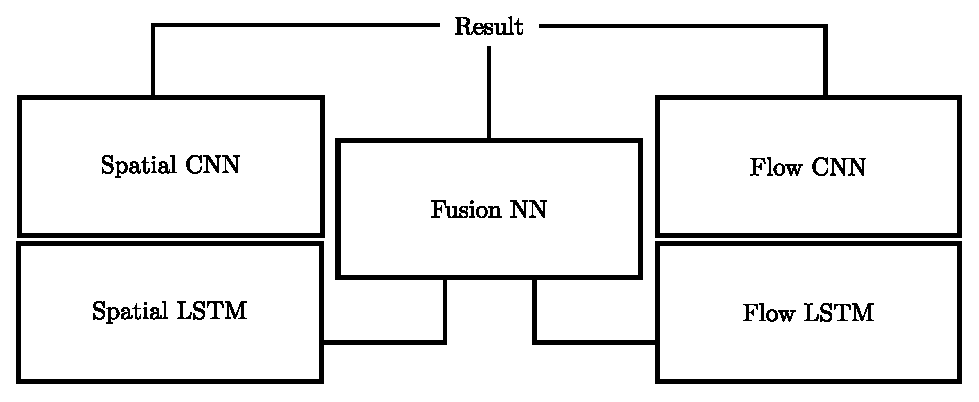
\includegraphics[scale=.7]{images/architecture.eps}
	\caption{General Architecture TODO}
	\label{fig:architecture}
\end{figure}

The individual neural networks used in this architecture differ from the work of ...\todo{reference}.
During our research we tried out different neural networks for the two streams, which will be presented in this section.
Also the parameters, which were used for the training, and the results will be shown.

\subsection{Changes to Caffe-tmbo}

\begin{itemize}
	\item New sequence data layer
	\item Multi-layer script
	\item More?
\end{itemize}

\subsection{Spatial}
\label{subsec:spatial}

\begin{itemize}
	\item
		Different nets:
		\begin{itemize}
			\item Caffenet/CNN\_M (also tried, VGG 19, but too big)
			\item With weights/without weights
			\item Compare the nets with respect to memory, number of parameters, training time, performance
		\end{itemize}
	\item
		Experiments:
		\begin{itemize}
			\item Different dropouts
			\item Train from scratch vs train from weights
			\item On different splits?
			\item Fc6, Fc7, fc8
			\item Different base data sets (only 16, all data)
			\item Different flows?
			\item Occlusion tests
		\end{itemize}
	\item
		LSTM did not work out
\end{itemize}


\subsection{Flow}
\label{subsec:flow}


\subsection{Fusion}
\label{subsec:fusion}
As first approach we rebuild the fusion architecture presented by TODO.

We took the CNN nets for spatial and flow presented above and build a fusion architecture on top of them.
Both CNNs were cut off after the \textit{fc6}-layer having an output of 16 x 4096.\todo{Der eigentlich output von fc6 ist ja erstmal 1 x 4096}
The input to the CNNs were 16 frames per video.
So the output of the \textit{fc6}-layer of the spatial and flow net correspond to a prediction for each of those frames.
To fuse those predictions, the first step is to merge the 16 prediction of one video into one prediction for the whole video.
Therefore, we take the average prediction for both spatial and flow.
A fully-connected layer is then trained with those predictions before we concatenate the predictions of spatial and flow.
In the end two fully-connected layer are trained on the merged predictions.
The output is defined by an accuracy layer.
The whole architecture is shown in Figure~\ref{fig:fusion_architecture}\todo{improve figure}.
\begin{figure}[!htb]
	\centering
	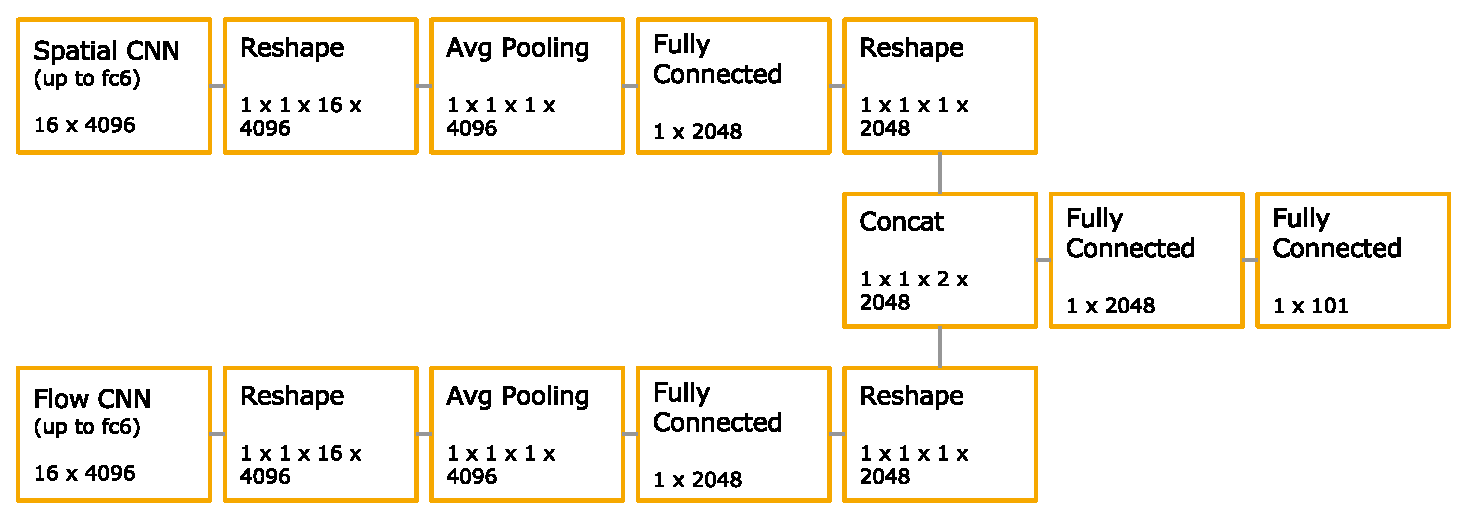
\includegraphics[scale=.7]{images/fusion_architecture.eps}
	\caption{Architecture of the fusion net: The predictions per frame of one video from the spatial and flow net are merged into one prediction per video each. Those predictions are then merged and trained via two fully connected layers.}
	\label{fig:fusion_architecture}
\end{figure}








%!TEX root = ../paper.tex
\section{Web Application}
\label{sec:web}

A web-based interface serves as an easily accessible interface to our classification system.
Users are given the opportunity to upload a video file as input for the prediction.
Alternatively, we provide example videos from the UCF-101 dataset for quick access.
The uploaded video material undergoes the same preprocessing as outlined in section \ref{sec:data}.
The extracted frames and optical flows serve as the input for the spatial and temporal network, respectively.
The joint prediction results are returned by means of a REST interface and are presented two-fold as shown in figure \ref{fig:web_app}:
\textit{(1)} Next to a preview of the video is the overall classification summary given by the top five label probabilities.
(\textit{2}) To reflect a video’s temporal dimension the demo presents a per-frame based evaluation highlighting the top five probabilities for each frame.
For easy verification a click on the graphical nodes synchronizes the preview video with the selected frame.

\begin{figure}[!htb]
	\centering
	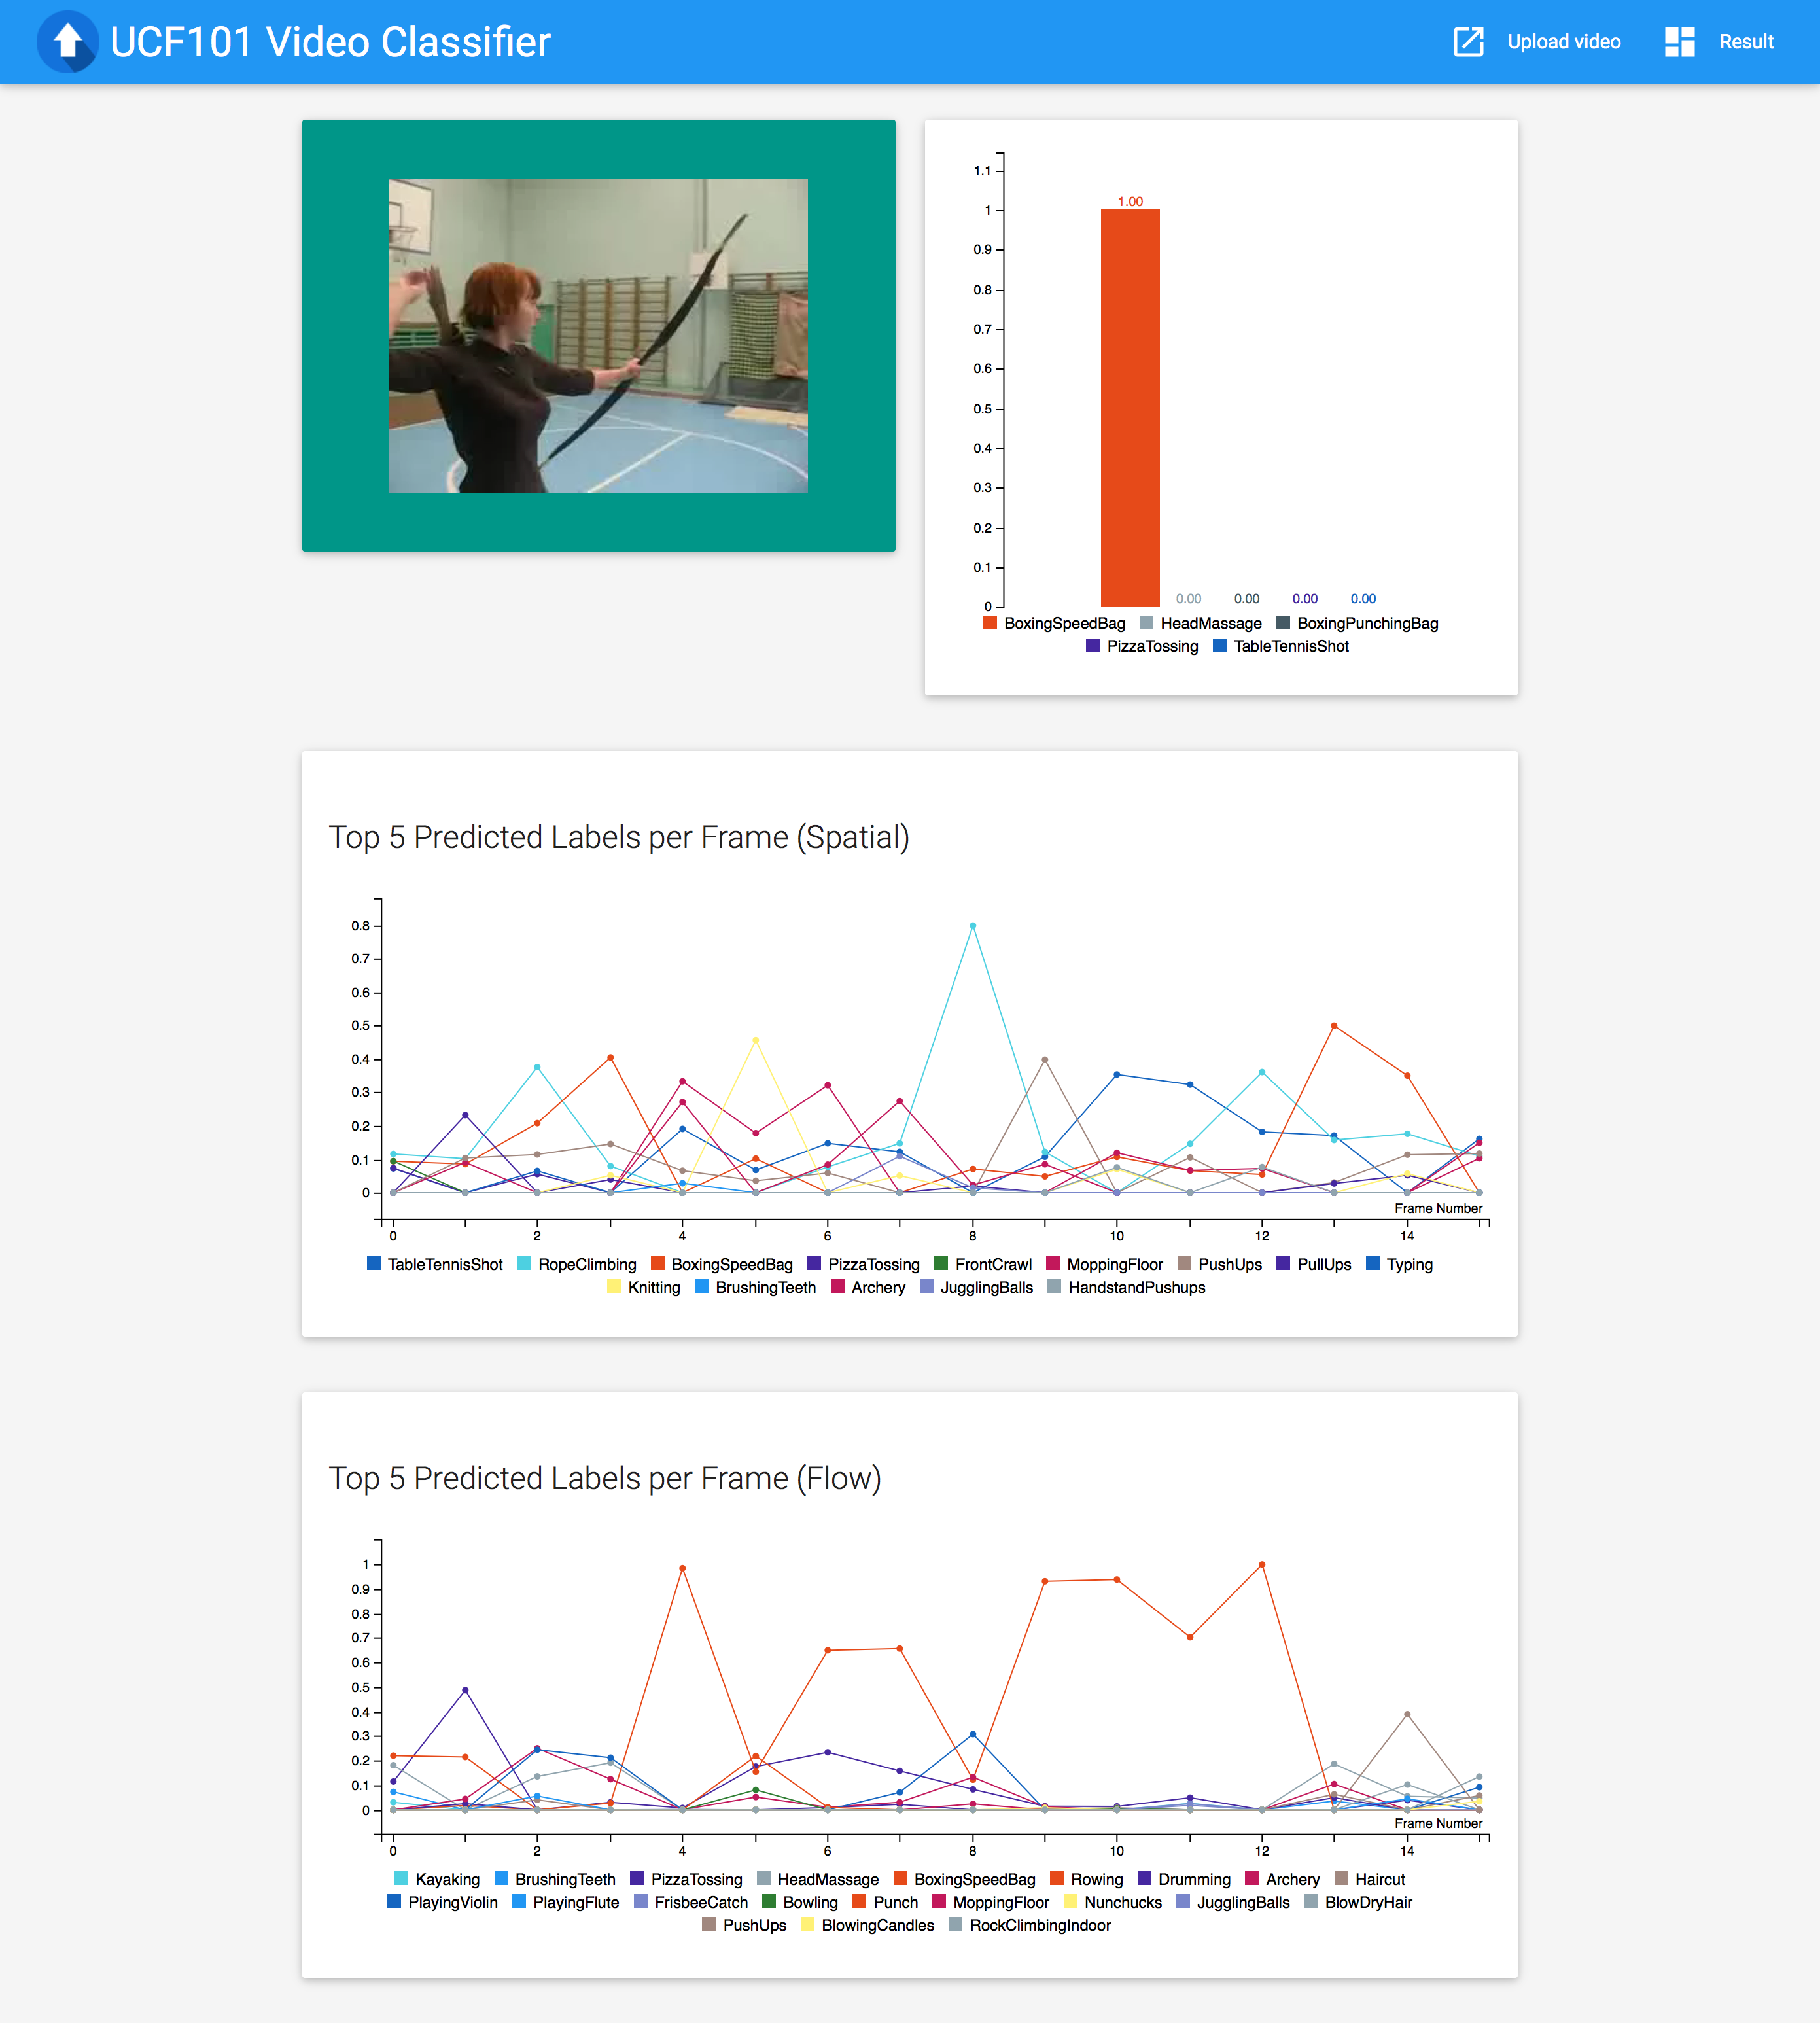
\includegraphics[width=0.9\textwidth]{images/screenshot.png}
	\caption{Visualization of the network's results: (Top) The video with the overall classification summary given by the top five label probabilities is given. (Middle) The per frame prediction of the \emph{spatial} neural network. (Bottom) The per frame prediction of the \emph{flow} neural network is shown.}
	\label{fig:web_app}
\end{figure}

\todo[inline]{Tausche Screenshot gegen einen mit besseren Ergebnissen!}

\subsection{Architecture}
The system contains of two almost independent parts:
(\textit{1}) A modern single-page web app.
The frontend utilizes the modular \textit{React}\footnote{\url{https://facebook.github.io/react}} UI-framework and follows the \textit{Flux} \footnote{\url{https://facebook.github.io/flux}} unidirectional data flow pattern.
Frontend routing, templating and interaction handling provides a rich and seamless experience.
In order to utilize the latest Javascript ES6 language-level features and retain backward compatibility with older browsers the frontend part has to be transpiled into a single file.
The scriptable module bundler \textit{Webpack} \footnote{\url{https://webpack.github.io}} takes care of that.

\textit{(2)} The server part is implemented in the Flask framework \footnote{\url{http://flask.pocoo.org}} for Python.
Besides providing an easy to modify web framework our choice for Python makes it easy to include Caffe through the PyCaffe bindings.
User videos are locally preproccessed using the same FFmpeg and OpenCV pipeline as outlined previously in section \ref{sec:data}.
After initially serving the web app to a client, all communication is then through a REST interface.

\subsection{Setup}
Make sure to install NodeJS, Python 2.7, OpenCV, PyCaffe and FFmpeg.
Listing \ref{lst:web-app} shows the required commands to install all further dependencies and run the server.

\begin{lstlisting}[language=sh, caption=Web Application Setup, label=lst:web-app]
cd web-server

# frontend dependencies
npm install -g webpack
npm install
npm run build

#server dependencies
pip install -r requirements.txt

#run the server
python server.py
\end{lstlisting}

%!TEX root = ../paper.tex
\section{Scripts and their Usage}
\label{sec:scripts}

During the project we wrote scripts for several use cases.
These scripts are listed below.
All scripts can be found on the server \texttt{fb10dl03}.

\subsection{frame\_extraction.sh}
This script extracts frames from videos in a specific frame rate.

\begin{table}[ht]
\begin{tabular}{lll}
\multicolumn{2}{l}{Location}  & \textit{/home/mpss2015m\_1/video-classification/tools} \\
\multicolumn{2}{l}{Parameter} &                                        \\
        & \textit{input\_folder}       & the input folder containing the videos \\
        & \textit{output\_folder}      & the output folder                      \\
        & \textit{frame\_rate}         & the frame rate
\end{tabular}
\end{table}



\begin{itemize}
	\item Convert scripts
	\item Database creation, lmdb, leveldb, hdf5
	\item Experiment setup
\end{itemize}


\newpage
\begin{thebibliography}{1}

\bibitem{meinel2008}
C.~Meinel.
``Tele-Lab IT-Security: an Architecture for an online virtual IT Security Lab'',
\emph{International Journal of Online Engineering (iJOE)},
X, 2008.

\end{thebibliography}

\end{document}
